\documentclass{umemoria}
\usepackage{minted}
\usepackage{booktabs}
\usepackage{caption}
\usepackage{subcaption}
\usepackage{svg}
\usepackage{pdfpages}
\usepackage[]{biblatex}
\usepackage{pgf-pie}
\usepackage{algorithm}
\usepackage{algpseudocodex}
\usepackage{amsmath}

\renewcommand{\listingscaption}{Código}
\renewcommand{\listoflistingscaption}{Índice de Códigos}

\floatname{algorithm}{Algoritmo}
\renewcommand{\listalgorithmname}{Índice de Algoritmos}

\addbibresource{bibliografia.bib}

%% Uncomment for final version:
\usepackage{microtype}

\defaultfontfeatures{Scale=MatchLowercase}
\defaultfontfeatures[\rmfamily]{Ligatures=TeX,Scale=1}
\setmainfont{Minion 3}[
  Numbers={Proportional,Lining},
  UprightFeatures={
    SizeFeatures={
      {Size={-9},Font=*Caption},
      {Size={9-14},Font=*Regular},
      {Size={14.0-24},Font=*Subhead},
      {Size={24-},Font=*Display}
  }},
  ItalicFeatures={
    SizeFeatures={
      {Size={-9},Font=*Caption Italic},
      {Size={9-14},Font=*Italic},
      {Size={14.0-24},Font=*Subhead Italic},
      {Size={24-},Font=*Display Italic}
  }},
  BoldFeatures={
    SizeFeatures={
      {Size={-9},Font=*Caption Bold},
      {Size={9-14},Font=*Bold},
      {Size={14.0-24},Font=*Subhead Bold},
      {Size={24-},Font=*Display Bold}
  }},
  BoldItalicFeatures={
    SizeFeatures={
      {Size={-9},Font=*Caption Bold Italic},
      {Size={9-14},Font=*Bold Italic},
      {Size={14.0-24},Font=*Subhead Bold Italic},
      {Size={24-},Font=*Display Bold Italic}
  }},
  SmallCapsFeatures = {
    Letters = SmallCaps,
    LetterSpace = 10,
  }]
\setsansfont[]{Helvetica Neue}
\setmonofont[]{JetBrains Mono}

\AtBeginEnvironment{tabular}{\addfontfeature{Numbers={Uppercase,Monospaced}}}

\depto{Departamento de Ciencias de la Computación}
\author{José Luis Romero Munizaga}
\title{Librería de Visualización de Estructuras de Datos}

% incluir ambos comandos para una doble titulación
%  o quitar el comando que no aplica
\memoria{Ingeniero Civil en Computación}
% \tesis{Magíster en ???}
%\tesis{Doctor en ???} % incluir solo este comando para doctorados

% puede haber varios profesores guía seperados por coma;
% pero si es una memoria, solo puede haber un profesor guía
\guia{Ivan Sipiran Mendoza}

% puede haber varios profesores co-guía seperados por coma;
% pero si es una memoria, el profesor co-guía será el primer
% integrante de la comisión
%\coguia{Nombre Completo Co-Guía} % incluir en caso de co-guía de *tesis*

%\cotutela{Nombre Institución} % incluir en caso de cotutela

\comision{Dionisio González González,Federico Olmedo Berón}

%\auspicio{Nombre Institución} % incluir en caso de recibir financiamiento

% tiene que ser el año en que se da el examen de título/grado (defensa)
%\anho{2021} % incluir solo para reemplazar el año actual

\begin{document}

\frontmatter
\maketitle

\begin{resumen}
Las estructuras de datos son uno de los temas más importantes en las Ciencias de la Computación.
Por el mismo motivo son parte de los contenidos básicos que se enseñan en esta disciplina.
Frecuentemente en la docencia se utilizan diagramas de las estructuras de datos como un apoyo al aprendizaje, pero estos diagramas son estáticos y no capturan la naturaleza dinámica de las estructuras de datos.
Si bien, si existen visualizaciones animadas de estructuras de datos, estas son poco flexibles y están separadas del ambiente donde se implementan las estructuras de datos.

En particular, para el curso Algoritmos y Estructuras de Datos del Departamento de Ciencias de la Computación de la Universidad de Chile se desarrolló previamente una herramienta que genera diagramas estáticos y existe la necesidad de una herramienta similar, pero que permita generar visualizaciones animadas.

Por lo anterior, sería útil contar con una herramienta que permita generar visualizaciones animadas de estructuras de datos que esté incorporada en el mismo ambiente de desarrollo.
De esta manera, el usuario puede visualizar la estructura de datos al mismo tiempo que la implementa, incluso permitiéndole ver cuando su implementación tiene errores.

Para satisfacer esta necesidad se creó \textit{dsvisualizer}, una herramienta para generar visualizaciones animadas de estructuras de datos implementadas en Python.
En su versión actual solo permite visualizar listas enlazadas, pero está diseñada para permitir generar visualizaciones de más estructuras de datos en el futuro.
Le permite al usuario generar una animación de su propia implementación, minimizando la intervención que debe realizarle a su código.

Para lograr esto, \textit{dsvisualizer} tiene un \textit{back-end} y un \textit{front-end}. El \textit{back-end}, implementado en Python, captura las operaciones sobre la estructura a visualizar y genera un modelo de estas que se lo envía al \textit{front-end}. Este, implementado en TypeScript, recibe el modelo desde el \textit{back-end} y a partir de este genera la visualización animada, utilizando la librería de animación D3js.

Para evaluar la herramienta se hicieron pruebas con usuarios ---12 estudiantes de la Facultad de Ciencias Físicas y Matemáticas---, donde se les pidió utilizar la herramienta y luego contestar un cuestionario. La primera parte de este corresponde a la escala de usabilidad SUS, en la cual la herramienta obtuvo un puntaje promedio de 90 de 100 puntos. La segunda parte consiste en preguntas abiertas, donde se preguntó por: comentarios positivos, comentarios negativos y oportunidades de mejora. El resultado de la evaluación fue muy positivo, pero de todas maneras se identificaron varias oportunidades de mejora y nuevas funcionalidades que contribuirían a hacer la herramienta aún más útil.
\end{resumen}

% opcional: incluir para tesis en inglés;
%  en este caso hay que tener el resumen y abstract
%   en ambos idiomas
%\begin{abstract}
%\lipsum[1-4]
%\end{abstract}

\begin{dedicatoria}
A los futuros estudiantes de Ciencias de la Computación.
\end{dedicatoria}

\begin{thanks}

Agradezco a Ivan Sipirán, por su excelente disposición, por sus sugerencias y por su apoyo como profesor guía durante todo el proceso de la memoria.

También quiero agradecer a todos los estudiantes que participaron de la evaluación y contribuyeron con su tiempo a mejorar esta herramienta.

Por otra parte, agradezco a mis amigos y a mi familia, por el ánimo, apoyo y ayuda que me han dado siempre y me dieron mientras trabajaba en la memoria.

% Agradezco a Ivan Sipirán, por su apoyo durante todo el proceso de la memoria como profesor guía.

% Agradezco a todos los estudiantes que contribuyeron con su tiempo participando de la evaluación.

% Agradezco a mi familia por la ayuda que me prestaron durante todos este proceso y por la que me han prestado siempre.
\end{thanks}

\setcounter{tocdepth}{1}
\tableofcontents
\listoffigures % opcional
\listoftables % opcional
% \listoflistings
% \listofalgorithms

\mainmatter

\chapter{Introducción}

Posiblemente uno de los temas más relevantes en las Ciencias de la Computación corresponde a las Estructuras de Datos. Las estructuras de datos son maneras de almacenar y organizar los datos para facilitar su acceso y modificación~\cite{Algorithms}. Comúnmente se utilizan diagramas y otras visualizaciones para facilitar la comprensión de las estructuras de datos y las operaciones que se realizan sobre ellas. En particular, las visualizaciones de estructuras de datos pueden ser útiles para la docencia en Ciencias de la Computación y pueden ser utilizadas tanto por los estudiantes como por los profesores. Las visualizaciones de algoritmos son efectivas para ayudar en el aprendizaje de estudiantes de Ciencias de la Computación~\cite{Hundhausen2002}.

Tradicionalmente, las visualizaciones de estructuras de datos que se utilizan son diagramas estáticos. Sin embargo, dado que las estructuras de datos son dinámicas y no estáticas, es útil utilizar visualizaciones que sean animaciones dinámicas de las estructuras de datos. Comúnmente las animaciones de estructuras de datos son videos o páginas web interactivas, pero en ambos casos desconectadas de donde se programan estas estructuras de datos. Por lo tanto, sería útil contar con una herramienta para generar visualizaciones animadas de estructuras de datos que se pueda usar al mismo tiempo que se implementan.

En los últimos años se ha vuelto más común la utilización de Jupyter Notebooks en la enseñanza de Ciencias de la Computación. Los Notebooks son ambientes de desarrollo interactivos basados en tecnologías web, que permiten combinar bloques de texto, bloques de código y los resultados generados por los bloques de código, para ser mostrados por una aplicación web interactiva que permite correr los bloques de código y ver los resultados generados por esto, que pueden incluir texto, imágenes, animaciones y elementos interactivos~\cite{kluyver2016jupyter}. Originalmente fueron diseñados para ser utilizados en el ámbito de la Ciencia de los Datos, pero han estado tomando popularidad en otras áreas de la computación y en la docencia.

El lenguaje de programación Python es un lenguaje de alto nivel, multiparadigma, de uso general y usualmente interpretado que se ha vuelto uno de los lenguajes más populares. Según la encuesta realizada anualmente por GitHub es el segundo lenguaje más popular, solo siendo superado por el lenguaje de programación JavaScript~\cite{encuesta-github}. Además, probablemente es uno de los lenguajes más utilizados en la docencia de Ciencias de la Computación.

Dada la popularidad de los Jupyter Notebooks y del lenguaje de programación Python, especialmente en docencia, sería beneficioso contar con una herramienta para generar visualizaciones animadas de estructuras de datos que se pueda usar en Jupyter Notebooks en el lenguaje de programación Python. De esta manera se aprovecha que los Jupyter Notebooks, a diferencia de otros ambientes de desarrollo, permite generar elementos interactivos usando las tecnologías web.

En particular, en el curso de Algoritmos y Estructuras de Datos de la Facultad de Ciencias Físicas y Matemáticas (FCFM) de la Universidad de Chile se utiliza tanto Python, como Jupyter Notebooks y se desarrolló una librería para generar visualizaciones de estructuras de datos. Esta librería tiene como objetivo de ayudar en la docencia permitiéndole tanto a los alumnos como a los profesores generar visualizaciones de estructuras de datos implementadas por ellos, por el profesor, o por algún libro o recurso externo. Sin embargo, esta librería actualmente cuenta con una serie de limitaciones: La implementación no es tan eficiente como podría ser, la API (Application Programming Interface) que se utiliza para usar la herramienta no es muy ergonómica y no permite visualizar cómo se ejecutan las operaciones sobre las estructuras de datos (solo permite visualizar una estructura de datos en un momento en el tiempo).

El problema abordado consiste en implementar una herramiento que permita generar visualizaciones animadas de las operaciones que se realizan sobre una estructura de datos implementada por el usuario. Para esto la herramiento debe ser capaz de registrar las operaciones sobre la estructura y debe ser capaz de generar una visualización animada a partir de las operaciones que registró. Es deseable que la visualización se genere en el mismo notebook y que el usuario tenga que agregar la menor cantidad de instrumentación a su código para que la herramienta funcione.

Implementar una librería que cumpla con estos requerimientos sería beneficioso para estudiantes de ciencias de la computación, profesores o personas en general, que estén aprendiendo estructuras de datos, o que deseen generar visualizaciones de estructuras de datos implementadas en Python y verlas en Jupyter Notebooks. Además, concretamente permitiría contribuir a la docencia en el curso Algoritmos y Estructuras de Datos de la FCFM.

Para lograr esto se implementó la herramienta \textit{dsvisualizer}, una librería de Python que genera visualizaciones animadas de estructuras de datos implementadas por los usuarios en Jupyter Notebooks. En su versión actual se limita a listas enlazadas, pero está diseñada para poder expandirla a otras estructuras de datos. La herrmienta está implementada como un Jupyter Widget con un backend escrito en Python que se encarga de registrar las operaciones realizadas por el usuario y un frontend escrito en JavaScript que genera las visualizaciones usando las operaciones registradas por el backend. Las dos partes de la herramiento se comunican usando la librería ipywidgets, que usa tecnologías web para mantener modelos sincronizados en el frontend y el backend.

\chapter{Estado del Arte}


\section{Librerías de visualización de estructuras de datos}

Actualmente existen varias librerías para generar visualizaciones de estructuras de datos, pero muchas de ellas están implementadas en lenguajes distintos de Python y no están diseñadas para poder ser utilizadas en Notebooks.
Un ejemplo de esto es la librería Reftree~\cite{Stanch2021} que permite crear visualizaciones de estructuras de datos, pero en el lenguaje Scala, por lo tanto, no se puede utilizar para visualizar estructuras de datos implementadas en Python y tampoco se puede utilizar en Jupyter Notebooks.
Otro ejemplo es la librería Lolviz~\cite{Lolviz} que, si bien si permite visualizar en Notebooks estructuras de datos implementadas en Python, cuenta con la limitación de que no puede generar animaciones. En la figura \ref{fig:comparacion} se pueden ver ejemplos de las visualizaciones generadas por estas librerías.

\begin{figure}[h]%
    \centering
    \subfloat[Reftree]{
        \centering
        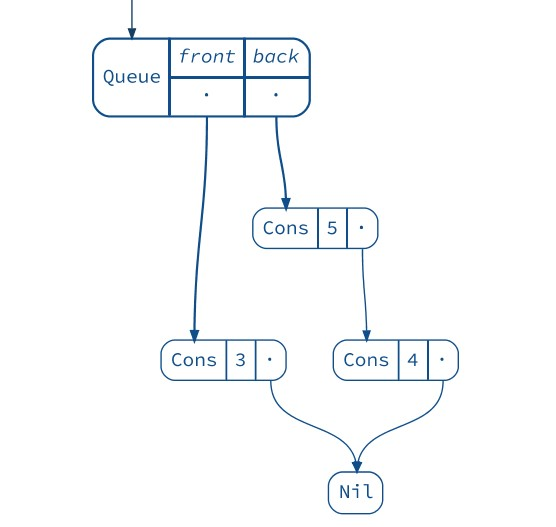
\includegraphics[width=\dimexpr(\linewidth-12pt)/2\relax, height=\dimexpr(\linewidth-12pt)/2\relax]{imagenes/ejemplos/reftree}
        \label{fig:reftree}
    }
    \subfloat[Lolviz]{
        \centering
        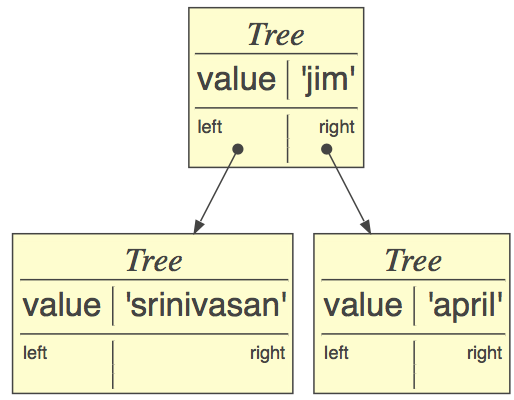
\includegraphics[width=\dimexpr(\linewidth-12pt)/2\relax]{imagenes/ejemplos/lolviz}
        % \vspace{38px}
        \label{fig:lolviz}
    }\\
    \subfloat[Aed Utilities]{
        \centering
        \includesvg[width=\dimexpr(\linewidth-12pt)/2\relax]{imagenes/ejemplos/aed}
        \label{fig:aed}
    }
    \subfloat[Manim]{
        \centering
        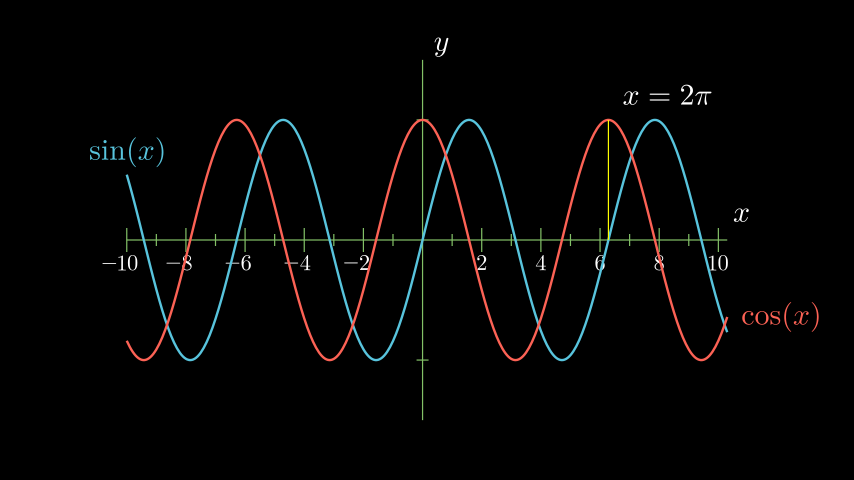
\includegraphics[width=\dimexpr(\linewidth-12pt)/2\relax]{imagenes/ejemplos/manim}
        \label{fig:manim}
    }
    \caption[Ejemplos de las distintas herramientas.]{Ejemplos de visualizaciones generadas por las distintas herramientas. Obtenidas de \cite{Stanch2021}, \cite{Lolviz}, \cite{aed-utilities} y \cite{manim}, respectivamente.}
    \label{fig:comparacion}
\end{figure}

Por otro lado, existe la librería Aed-Utilities~\cite{aed-utilities} creada para el curso de Algoritmos y Estructuras de Datos de la FCFM por el Profesor Ivan Sipiran; que, si bien permite generar diagramas de estructuras de datos en Python y mostrarlas en un Notebook, cuenta con las siguientes limitaciones: no permite crear animaciones, la API no es muy cómoda de utilizar y el algoritmo que utiliza para generar las visualizaciones es poco eficiente. % TODO: Explicar

Tanto Aed-Utilites como Lolviz generan los diagramas utilizando Graphviz ---una herramienta originalmente desarrollada por AT\&T para dibujar gráficos especificados en el lenguaje DOT--- que permite generar diagramas de muy buena calidad, pero no permite crear animaciones.

En cuanto a las herramientas para generar animaciones, existe la librería Manim~\cite{manim}, diseñada para generar visualizaciones animadas de matemáticas. Si bien no está diseñada para crear visualizaciones de estructuras de datos, es relevante porque permite generar animaciones y estas animaciones se pueden ver desde Notebooks. Esta librería tiene un diseño orientado a objetos, donde una animación es un objeto que tiene un campo con el objeto matemático que representa y tiene un método que permite animar el objeto según una función de interpolación. Para generar el resultado final puede utilizar varios back-ends de rendering, incluyendo OpenGL y WebGL. Utilizando este último cuando se usa desde un Notebook. En la figura \ref{fig:manim} se puede ver una visualización de una función creada con esta herramienta.

Otra herramienta enfocada en las matemáticas es Penrose~\cite{Penrose}, una herramienta que permite crear diagramas a partir de un programa en un lenguaje específico de dominio. La disposición de los elementos en el diagrama se obtiene mediante optimización numérica. El lenguaje específico de dominio (o DSL por sus iniciales en inglés) se separa en un archivo que define solo la parte matemática y en otro que define el estilo.

Dado que no se encontró ninguna herramienta existente que permita visualizar estructuras de datos implementadas en Python, permita generar animaciones y permita mostrar las visualizaciones generadas en un Jupyter Notebooks, se requiere crear una nueva librería que implemente esta funcionalidad.

\section{Jupyter Notebooks}

Los Jupyter Notebooks son archivos interactivos que almacenan bloques de texto, código y también pueden contener imágenes, videos y animaciones interactivas. Un Jupyter Notebook tiene varios componentes que permiten construir la experiencia de usuario. En primer lugar, está el archivo del notebook que es un archivo JSON con la extensión \texttt{.ipynb}, que almacena en el disco todos los datos persistentes del notebook, incluyendo los bloques de texto, los bloques de código y sus salidas, las imágenes, etc. Después, está el \textit{kernel} o núcleo, que es un intérprete del lenguaje respectivo, con la capacidad de comunicarse con el servidor del notebook. El servidor del notebook se encarga de la comunicación entre el front--end, el kernel y el archivo del notebook. Finalmente, está el front--end del notebook, que se encarga de mostrarle al usuario una representación del notebook y le permite a este interactuar con el notebook, usualmente corresponde a un navegador web. En la figura \ref{fig:notebook_arq} se puede ver un diagrama de esta arquitectura.

\begin{figure}[h]
  \centering
  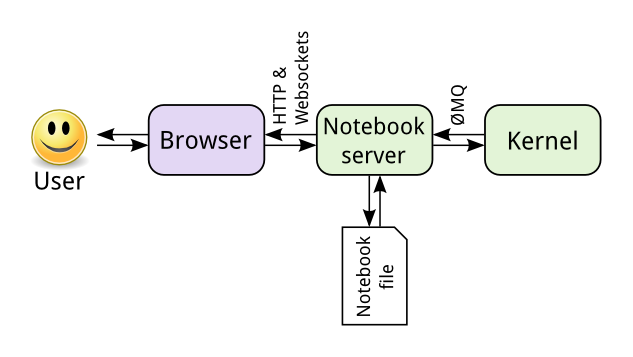
\includegraphics[width=0.8\linewidth]{imagenes/notebook/notebook_components}
  \caption[Arquitectura de Jupyter Notebooks]{Arquitectura de Jupyter Notebooks. Obtenido de \cite{arq-notebook}.}
  \label{fig:notebook_arq}
\end{figure}

Existen múltiples kernels, uno por cada lenguaje que soportan los Jupyter Notebooks, pero el más conocido es el kernel IPython que es el kernel del lenguaje Python. IPython además de ser un kernel de Jupyter Notebooks es un intérprete interactivo de Python, con funcionalidades como contenido multimedia y completado de comandos. Cuando se utiliza un notebook con el lenguaje Python, el servidor del notebook se comunica con este intérprete que es que se encarga de interpretar los bloques de código y responder con la salida generada cuando el servidor del notebook envía el request.

Para crear componentes interactivos en un Notebook de Python se utiliza la librería Jupyter Widgets. Esta librería permite definir un modelo que representa el componente, y una vista en JavaScript y HTML que es mostrada por el front--end del Notebook. El modelo se define tanto en JavaScript como en Python y la librería se encarga de mantener las dos versiones sincronizadas. Para mantener las dos versiones sincronizadas, es necesario serializar y deserializar los campos del modelo, para poder enviarlos en formato JSON. Entonces, para los campos sencillos, la librería se puede encargar de la serialización o deserialización, pero para los casos más complejos se deben definir manualmente los serializadores y deserializadores para cada campo. En la figura \ref{fig:widget_arq} se observa la arquitectura de un widget generado con esta librería.

\begin{figure}[h]
  \centering
  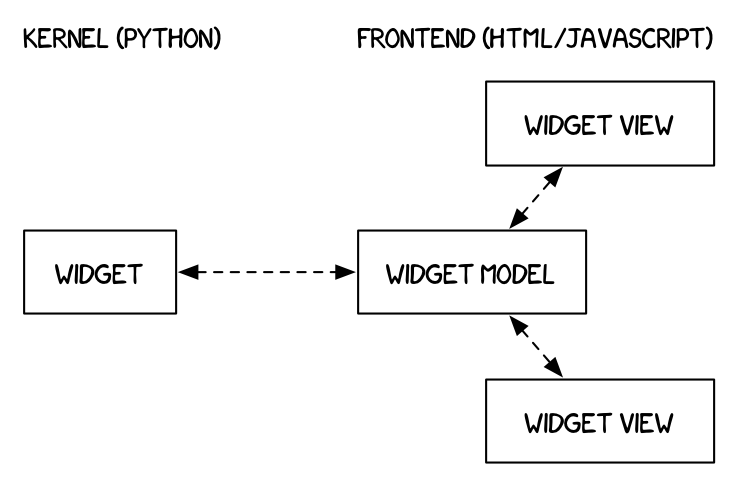
\includegraphics[width=0.8\textwidth]{imagenes/notebook/WidgetModelView}
  \caption[Arquitectura de Jupyter Widgets]{Arquitectura de Jupyter Widgets. Obtenido de \cite{arq-widget}.}
  \label{fig:widget_arq}
\end{figure}

\section{D3}

D3 es una librería de JavaScript para manipular documentas en función de datos. Esta librería permite manipular el DOM (Document Object Model) y aplicarle transformaciones según los datos. Permite usar las tecnologías estándar de la web para generar visualizaciones de buena calidad.

Es particularmente útil la capacidad de D3 de manipular elementos SVG (Scalable Vector Graphics) ---un lenguaje de markup para describir gráficos en dos dimensiones---. Esto permite generar animaciones en dos dimensiones de forma relativamente simple. Además esta técnica es bastante eficiente gracias a que los navegadores implementan motores muy eficientes para la renderización de elementos SVG.

Para lograr esto D3 permite enlazar datos con elementos del DOM y definir los atributos de estos elementos como función de los datos. Además, cuando cambian los datos se puede hacer una transición suave de los elementos correspondientes a su nueva posición según la función definida anteriormente. La figura~\ref{fig:d3-ejemplo} muestra un ejemplo de una visualización generada con D3 que representa un conjunto de datos como una agrupación de círculos.

\begin{figure}[h]
    \centering
    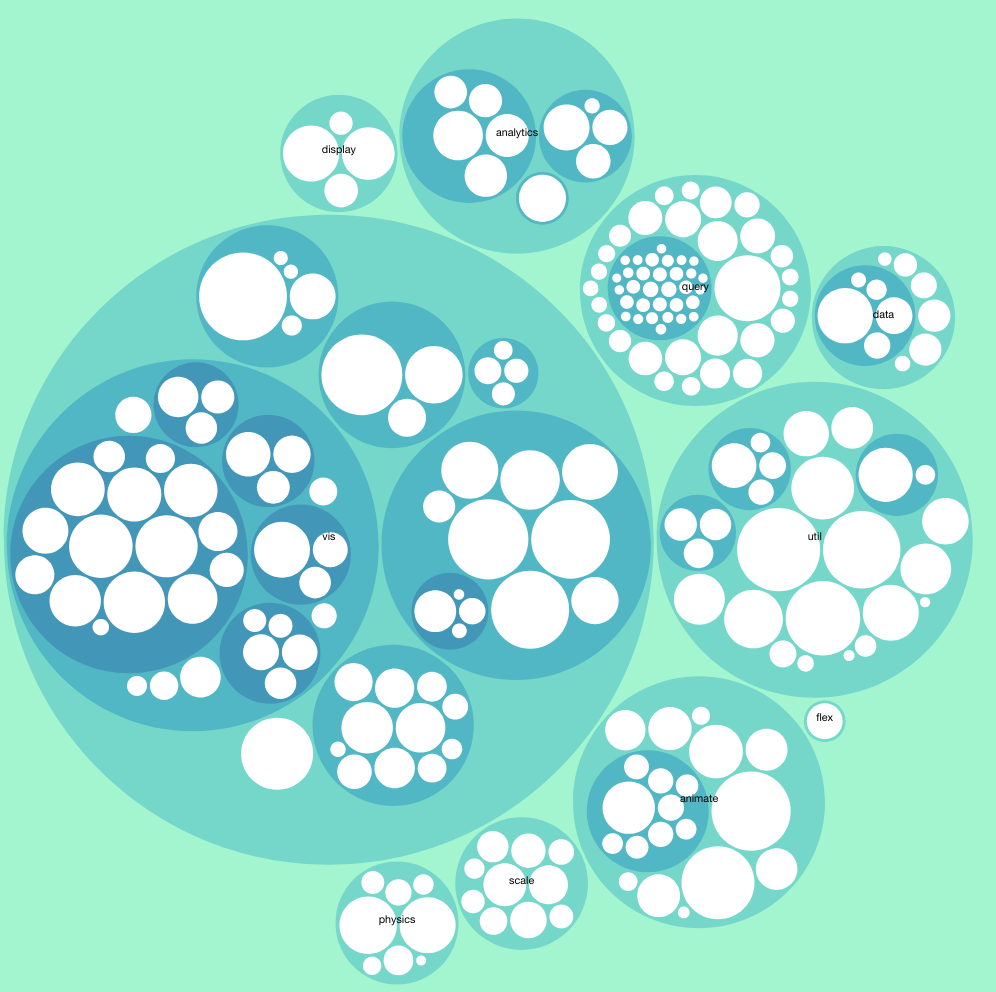
\includegraphics[width=\textwidth]{imagenes/d3/ejemplo.png}
    \caption{Ejemplo de visualización generada con D3}
    \label{fig:d3-ejemplo}
\end{figure}

\chapter{Problema}

%%%%%%%%%%%%%%%%%%%%%%%%%%%%%%%%%%%%%%%%%%%%%%%%%%%%%%%%%%%%%%%%%%%%%%%%%%%%%%%%%
%%% TODO: Expandir esta sección, por ahora es lo mismo que en la introducción %%%
%%%%%%%%%%%%%%%%%%%%%%%%%%%%%%%%%%%%%%%%%%%%%%%%%%%%%%%%%%%%%%%%%%%%%%%%%%%%%%%%%

% El problema abordado consiste en implementar una herramienta que permita generar visualizaciones animadas de las operaciones que se realizan sobre una estructura de datos implementada por el usuario. Para esto la herramienta debe ser capaz de registrar las operaciones sobre la estructura y debe ser capaz de generar una visualización animada a partir de las operaciones que registró. Es deseable que la visualización se genere en el mismo notebook y que el usuario tenga que agregar la menor cantidad de instrumentación a su código para que la herramienta funcione.

% Implementar una librería que cumpla con estos requerimientos sería beneficioso para estudiantes de ciencias de la computación, profesores o personas en general, que estén aprendiendo estructuras de datos, o que deseen generar visualizaciones de estructuras de datos implementadas en Python y verlas en Jupyter Notebooks. Además, concretamente permitiría contribuir a la docencia en el curso Algoritmos y Estructuras de Datos de la FCFM.

%%%%%%%%%%%%%%%%%%%%%%%%%%%%%%%%%%%%%%%%%%%%%%%%%%%%%%%%%%%%%%%%%%%%%%%%%%%%%%%%%

Tradicionalmente, las visualizaciones de estructuras de datos que se utilizan son diagramas estáticos. Sin embargo, dado que las estructuras de datos son dinámicas y no estáticas, es útil utilizar visualizaciones que sean animaciones dinámicas de las estructuras de datos. Comúnmente las animaciones de estructuras de datos son videos o páginas web interactivas, pero en ambos casos, desconectadas de donde se programan estas estructuras de datos. Por lo tanto, sería útil contar con una herramienta para generar visualizaciones animadas de estructuras de datos que se pueda usar al mismo tiempo que se implementan.

En los últimos años se ha vuelto más común la utilización de Jupyter Notebooks en la enseñanza de Ciencias de la Computación. Los Notebooks son ambientes de desarrollo interactivos basados en tecnologías web, que permiten combinar bloques de texto, bloques de código y los resultados generados por los bloques de código, para ser mostrados por una aplicación web interactiva que permite correr los bloques de código y ver los resultados generados por esto, que pueden incluir texto, imágenes, animaciones y elementos interactivos~\cite{kluyver2016jupyter}. Originalmente fueron diseñados para ser utilizados en el ámbito de la Ciencia de los Datos, pero han estado tomando popularidad en otras áreas de la computación y en la docencia.

El lenguaje de programación Python es un lenguaje de alto nivel, multiparadigma, de uso general y usualmente interpretado que se ha vuelto uno de los lenguajes más populares. Según la encuesta realizada anualmente por GitHub es el segundo lenguaje más popular, solo siendo superado por el lenguaje de programación JavaScript~\cite{encuesta-github}. Además, probablemente es uno de los lenguajes más utilizados en la docencia de Ciencias de la Computación.

Dada la popularidad de los Jupyter Notebooks y del lenguaje de programación Python, especialmente en docencia, sería beneficioso contar con una herramienta para generar visualizaciones animadas de estructuras de datos que se pueda usar en Jupyter Notebooks en el lenguaje de programación Python. De esta manera se aprovecha que los Jupyter Notebooks, a diferencia de otros ambientes de desarrollo, permite generar elementos interactivos usando las tecnologías web.

En particular, en el curso de Algoritmos y Estructuras de Datos de la Facultad de Ciencias Físicas y Matemáticas (FCFM) de la Universidad de Chile se utiliza tanto Python, como Jupyter Notebooks y se desarrolló una librería para generar visualizaciones de estructuras de datos. Esta librería tiene como objetivo de ayudar en la docencia permitiéndole tanto a los alumnos como a los profesores generar visualizaciones de estructuras de datos implementadas por ellos, por el profesor, o por algún libro o recurso externo. Sin embargo, esta librería actualmente cuenta con una serie de limitaciones: La implementación no es tan eficiente como podría ser, la API (Application Programming Interface) que se utiliza para usar la herramienta no es muy ergonómica y no permite visualizar cómo se ejecutan las operaciones sobre las estructuras de datos (solo permite visualizar una estructura de datos en un momento en el tiempo).

El problema abordado consiste en implementar una herramienta que permita generar visualizaciones animadas de las operaciones que se realizan sobre una estructura de datos implementada por el usuario. Para esto la herramienta debe ser capaz de registrar las operaciones sobre la estructura y debe ser capaz de generar una visualización animada a partir de las operaciones que registró. Es deseable que la visualización se genere en el mismo notebook y que el usuario tenga que agregar la menor cantidad de instrumentación a su código para que la herramienta funcione.

Implementar una librería que cumpla con estos requerimientos sería beneficioso para estudiantes de ciencias de la computación, profesores o personas en general, que estén aprendiendo estructuras de datos, o que deseen generar visualizaciones de estructuras de datos implementadas en Python y verlas en Jupyter Notebooks. Además, concretamente permitiría contribuir a la docencia en el curso Algoritmos y Estructuras de Datos de la FCFM.

\chapter{Solución}

\section{Arquitectura}

La solución es una librería de Python para generar visualizaciones animadas de estructuras de datos y las operaciones que se realizan sobre estas, que pueda ser usada en Jupyter Notebooks.

La librería le permite al usuario implementar una estructura de datos y, agregando la instrumentación provista por la librería, le permite generar una visualización animada de las operaciones que se realizaron sobre la estructura.

Para permitir esto la librería está compuesta por dos partes: el \textit{back-end} y el \textit{front-end}. Estas dos partes se comunican entre sí utilizando un modelo de datos común que cada una de las partes sabe serializar y deserializar.

\begin{figure}[htb]
    \centering
    \includesvg[width=\textwidth]{imagenes/diagramas/arquitectura.svg}
    \caption{Diagrama de la arquitectura}
    \label{fig:diagrama-arq}
\end{figure}

El \textit{back-end}, implementado en Python, define la instrumentación para capturar las operaciones realizadas sobre la estructura de datos. Se encarga de mantener un registro de todas las operaciones que se realizan sobre esta. Este registro se mantiene utilizando una representación de las operaciones primitivas sobre la estructura de datos. Teniendo esto, cuando un usuario quiere generar la visualización, este registro de operaciones es serializado y enviado al \textit{front-end}. Esto se logra utilizando usando la librería IPython Widgets en combinación con el serializador definido para el modelo.

El \textit{front-end}, implementado en TypeScript, recibe el modelo serializado, deserializa el modelo y genera la visualización a partir de este. Para generar la visualización utiliza la librería D3js, que permite manipular el DOM (Document Object Model) en función de los datos del modelo.

La figura~\ref{fig:flujo-informacion} es un diagrama que muestra el flujo de la información cuando se utiliza la herramienta. Primero el usuario implementa y usa la estructura de datos en el notebook, después a partir de esto se genera un registro en el back-end, luego este registro se sincroniza con el front-end y finalmente este último genera la animación en el navegador.

\begin{figure}[htb]
    \centering
    \includesvg[pretex=\footnotesize,width=\textwidth]{imagenes/diagramas/diagrama-de-flujo.svg}
    \caption{Flujo de la información}
    \label{fig:flujo-informacion}
\end{figure}

En la figura~\ref{fig:diagrama-arq} se puede ver un diagrama que representa la arquitectura física de la solución. El usuario interactúa con la herramienta usando el navegador, donde corre el front-end. Este se comunica usando HTTP y Websockets con el servidor de Notebooks, que se encarga de interactuar con el archivo del Notebook y se comunica con el kernel usando ZeroMQ ---una librería de comunicación asíncrona orientada a mensajes---. El kernel contiene el intérprete de Python y es donde corre el back-end de la herramienta.

\section{Modelo de datos}

Cuando un usuario quiere generar una visualización el back-end le envía al front-end una representación de las operaciones realizadas sobre la estructura de datos. Para esto se diseñó un modelo que representa las operaciones primitivas que se pueden realizar sobre las listas enlazadas. Además, el modelo contiene metadatos que son útiles para generar la visualización.

El modelo que se utiliza para generar la visualización consiste en una lista de operaciones y metadatos de la visualización. Cada operación consiste en una operación primitiva y metadatos de la operación.

Las operaciones primitivas son las siguientes:
\begin{itemize}
    \item{\makebox[3.5cm]{Init(id, value, next)\hfill}}: Inicializar un nodo
    \item{\makebox[3.5cm]{SetValue(id, value)\hfill}}: Asignar el valor de un nodo
    \item{\makebox[3.5cm]{GetValue(id)\hfill}}: Obtener el valor de un nodo
    \item{\makebox[3.5cm]{SetNext(id, next)\hfill}}: Asignar el siguiente de un nodo
    \item{\makebox[3.5cm]{GetNext(id)\hfill}}: Obtener el siguiente de un nodo
\end{itemize}
donde \textit{id} es el identificador único de cada nodo, \textit{value} es una cadena de texto que representa el valor del nodo y \textit{next} es el identificador del siguiente nodo en la lista enlazada o es \textit{null}.

Los metadatos de la visualización son configuraciones de la visualización, por ejemplo, la duración de las transiciones y la duración de los fade-ins y fade-outs. En cambio, los metadatos de las operaciones contienen información que solo es relevante para esa operación, por ejemplo, si se debe animar o no esa operación y el código fuente que dio origen a la operación.

En la figura~\ref{fig:codigo-vs-modelo} se puede ver un ejemplo de código fuente que usa la herramienta, una captura de la animación generada a partir de ese código y el modelo generado a partir del código que se usa para crear la visualización.

\begin{figure}[p]
    \centering
    \begin{subfigure}[b]{0.49\textwidth}
        \centering
        \begin{minted}[linenos=false,fontsize=\scriptsize]{python}
@node('value', 'next')
class Node:
    def __init__(self, value, next=None):
        self.value = value
        self.next = next

@container(lines_before=0, lines_after=0)
class List:
    def __init__(self):
        self.node = None
        
    def append(self, value):
        node = self.node
        if node is None:
            self.node = Node(value, None)
            return

        next = node.next
        while next is not None:
            node = next
            next = next.next
        node.next = Node(value, None)

l = List()
l.append(1)
l.append(2)
l.visualize()
        \end{minted}
        \caption{Código}
        \label{fig:codigo-vs-modelo:codigo}
    \end{subfigure}
    \hfill
    \begin{subfigure}[b]{0.49\textwidth}
        \centering
        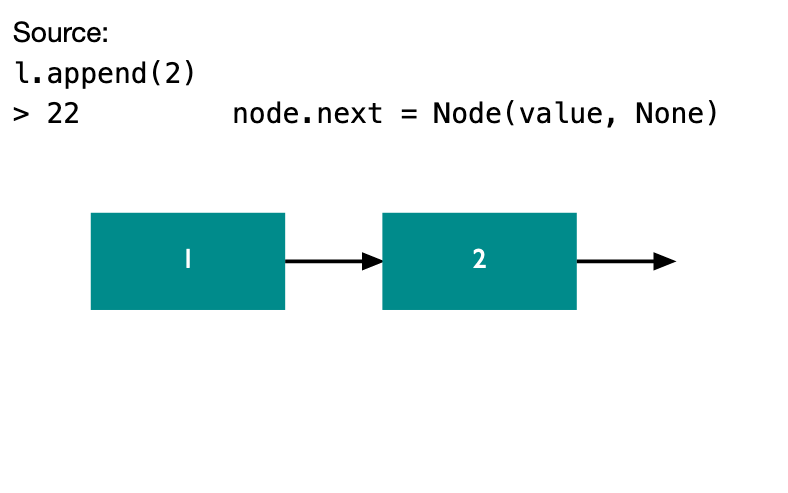
\includegraphics[width=\textwidth]{imagenes/codigo-imagen-modelo.png}
        \caption{Captura de la visualización}
        \label{fig:codigo-vs-modelo:imagen}
    \end{subfigure}
    \begin{subfigure}[b]{0.8\textwidth}
        \centering
        \begin{minted}[linenos=false,fontsize=\scriptsize]{json}
{
  "operations": [
    {
      "operation": { "operation": "init", "id": 6, "value": "1", "next": null },
      "metadata": {
        "animate": true,
        "source": ["l.append(1)\n", "> 15     self.node = Node(value, None)\n"]
      }
    },
    {
      "operation": { "operation": "get_next", "id": 6 },
      "metadata": {
        "animate": true,
        "source": ["l.append(2)\n", "> 18 next = node.next\n"]
      }
    },
    {
      "operation": { "operation": "init", "id": 7, "value": "2", "next": null },
      "metadata": {
        "animate": true,
        "source": ["l.append(2)\n", "> 22 node.next = Node(value, None)\n"]
      }
    },
    {
      "operation": { "operation": "set_next", "id": 6, "next": 7 },
      "metadata": {
        "animate": true,
        "source": ["l.append(2)\n", "> 22 node.next = Node(value, None)\n"]
      }
    }
  ],
  "metadata": { "transition_duration": 1000, "fade_in_duration": 1000 }
}
                      
        \end{minted}
        \caption{Modelo generado a partir del código}
        \label{fig:codigo-vs-modelo:modelo}
    \end{subfigure}
    \caption{Código, captura de la visualización y modelo}
    \label{fig:codigo-vs-modelo}
\end{figure}

Este modelo en realidad representa un grafo dirigido con un grado máximo de 1. Este nivel de flexibilidad es necesario porque como la representación se genera a partir de un programa escrito por el usuario, este puede contener errores que hagan que la estructura de datos implementada no sea necesariamente una lista enlazada. Por ejemplo, por ejemplo, el usuario puede crear nodos que no estén conectados entre sí y puede crear ciclos.

Para una versión futura de la herramienta se podría cambiar esta representación para que represente grafos sin un grado máximo. Esto permitiría representar estructuras de datos tales como grafos, árboles y listas enlazadas. Se consideró utilizar esta representación desde un principio, pero no se hizo porque dificultaba la generación de la visualización para la estructura de datos abordada.

\section{Back-end}

El back-end se encarga de proveer la instrumentación necesaria para que el usuario pueda generar visualizaciones de las estructuras de datos que ha implementado. Usando esta instrumentación mantiene un registro de las operaciones primitivas realizadas sobre la estructura de datos y cuando el usuario quiere visualizar el resultado serializa este registro y lo envía al \textit{front-end}.

Para esto la librería provee dos \textit{decoradores} ---azúcar sintáctica de Python para aplicar funciones a las definiciones de clases o funciones--- \textit{node} y \textit{container}. El primero de estos denota la clase que representa el nodo de la lista enlazada, mientras que el segundo denota la clase que contiene una referencia al primer nodo de la lista. En el código~\ref{lst:ejemplo-uso} se puede ver un ejemplo del uso de estos decoradores y en la figura~\ref{fig:visualizacion_ej} se puede ver un cuadro de la visualización generada.

\begin{listing}[htb]
\caption{Ejemplo de uso de la librería}
\label{lst:ejemplo-uso}
\begin{minted}[linenos=true]{python}
from dsvisualizer import node, container

@node('hd', 'tl')
class Node():
    def __init__(self, hd, tl):
        self.hd = hd
        self.tl = tl

@container()
class List():
    def __init__(self):
        self.head = None

    def push(self, v):
        self.head = Node(v, self.head)

l = List()
l.push(1)
l.push(2)
l.push(3)
l.visualize()
\end{minted}
\end{listing}

\begin{figure}[htb]
    \centering
    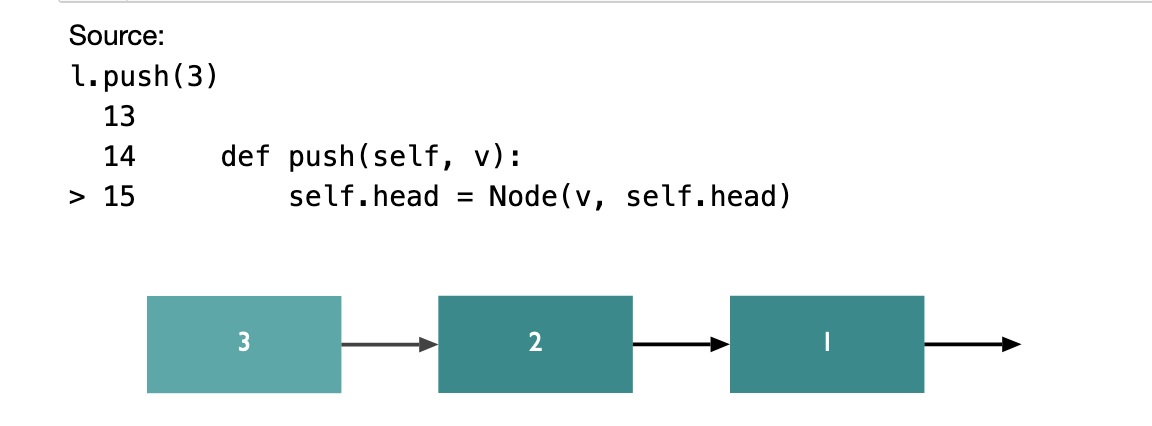
\includegraphics[width=\linewidth]{imagenes/ejemplos/ejemplo}
    \caption{Captura de la visualización generada a partir del código~\ref{lst:ejemplo-uso}.}
    \label{fig:visualizacion_ej}
    \centering
\end{figure}

Para registrar las operaciones primitivas sobre la estructura de datos el decorador \textit{node} modifica los campos pasados como parámetros para que al momento de acceder o asignar a estos campos se registre la operación en el \textit{logger}.

El \textit{logger} es un objeto que mantiene el registro de las operaciones primitivas sobre la estructura de datos. Además, se puede utilizar como un \textit{context manager} (objetos de Python que definen un contexto y se utilizan con \texttt{with}) y dentro del scope introducido todas las operaciones serán registradas en este \textit{logger}. En el código~\ref{lst:ejemplo-logger-ctx-mgr} se puede ver un ejemplo de esta funcionalidad.

\begin{listing}[htb]
\caption{Ejemplo de uso del \textit{logger} como un \textit{context manager}.}
\label{lst:ejemplo-logger-ctx-mgr}
\begin{minted}[linenos=true]{python}
from dsvisualizer import logger

with Logger() as logger:
    n = Node(5, Node(10, Node(20, None)))
logger.visualize()

with logger:
    n = Node(10, n)
logger.visualize()
\end{minted}
\end{listing}

Cuando se aplica el decorador \textit{container} a una clase, se crea un Logger asociado a cada instancia de esa clase y para todos los métodos de esa clase se utiliza ese logger como \textit{context manager} para que las operaciones sobre la estructura de datos queden registradas en el logger del contenedor.

Esta parte originalmente se implementó usando herencia en vez de decoradores, pero se cambió debido a que de esta manera eran menores los cambios que el usuario debía hacer a su programa para permitirle usar la herramienta.

\section{Front-end}

Como la librería registra las operaciones primitivas no es trivial generar una visualización a partir del modelo, ya que las operaciones registradas no necesariamente representan una operación estándar sobre listas. De hecho estas operaciones definen un grafo dirigido con un grado máximo de 1. Esta representación resulta útil porque permite representar implementaciones incorrectas de una lista enlazada.

Para visualizar por separado las componentes conexas del grafo se deben encontrar los subgrafos conexos a partir de esta representación. En la literatura existen varios algoritmos para resolver este problema, pero por simplicidad se decidió acotar la librería al caso donde el grafo es acíclico, es decir, un bosque. De esta manera, todos los nodos que no tienen ningún arco que apunte a ellos son puntos de entrada. Además, todos estos puntos de entrada definen una lista conexa que no tiene conexiones con otras listas. Entonces, podemos visualizar cada una de estas componentes conexas como una lista.

Para generar la animación se visualiza en orden cada operación primitiva que se obtiene del \textit{front-end} (animándola o no dependiendo de los metadatos de la operación). Para cada operación primitiva primero se obtienen las listas conexas usando el algoritmo descrito previamente, luego se genera una lista donde cada elemento tiene la información asociada a un nodo y finalmente usando D3js se anima la transición desde la versión previa de esta lista hasta la actual.

Los datos asociados a cada nodo son: el índice de la lista a la que pertenece, el largo de la lista a la que pertenece, su índice dentro de la lista a la que pertenece, su identificador único y su valor.

Teniendo la lista, usando D3js se asocian los nodos de la visualización a cada elemento en esta lista usando el identificador del elemento. La animación tiene dos fases: primero se anima la actualización de los nodos existentes y luego se anima la entrada de nuevos nodos.

En la primera fase se transiciona con una animación desde la posición anterior de los nodos a la posición dada por los datos actualizados asociados a cada nodo y se actualizan los valores que hayan cambiado. En la segunda fase se hace un \textit{fade in} de los nuevos nodos en las posiciones correspondientes. Es importante el orden de estas fases porque si se hace en otro orden los nodos entrantes podrían aparecer detrás de nodos preexistentes.

\section{Integración Continua y Entrega Continua}

Para que la herramienta pueda ser utilizada instalándola con el administrador de paquetes de Python se publicó en el repositorio oficial del administrador de paquetes de Python, PyPi (Python Package Index). Adicionalmente, cómo el front-end de la herramienta está implementado en TypeScript también fue necesario publicar un paquete en el repositorio NPM (Node Package Manager).

En el caso de Python generar el paquete es relativamente sencillo, porque solo utiliza el código definido en el archivo \texttt{setup.py}. En cambio, en el caso del TypeScript esto involucra el uso de una serie de herramientas. Algunas de estas herramientas son: el compilador de TypeScript (TSC) para el chequeo de tipos y la generación del código en JavaScript; y Webpack para generar \textit{bundles} minimizadas a partir del código en JavaScript obtenido de TSC. La generación de \textit{bundles} minimizadas es importante porque reduce el tamaño del paquete que tiene que instalar el usuario, lo que es especialmente relevante cuando este no cuenta con una buena conexión a internet, y porque reduce el tiempo inicial que el navegador se demora en poder ejecutar el código.

Para facilitar el lanzamiento de nuevas versiones de la herramienta el repositorio se encuentra en GitHub y utiliza Github Actions ---una funcionalidad de GitHub que permite ejecutar programas después de eventos como commits o deploys--- para correr las pruebas y para publicar versiones nuevas de la librería.

Cada vez que se agrega un commit al repositorio una GitHub Action corre los tests y los \textit{linters} de Python (Black) y de JavaScript (Prettier). Además, cuando se hace un release del repositorio otra Github Action compila los paquetes de Python y de JavaScript y los sube a los repositorios de los administradores de paquetes respectivos. Esto permite lanzar nuevas versiones de la herramienta de forma muy expedita, facilitando y acelerando el desarrollo.

\chapter{Validación}

\chapter{Conclusión}

% Breve resumen del trabajo realizado

Se desarrolló \textit{dsvisualizer}, una herramienta para generar visualizaciones animadas de estructuras de datos para ser utilizada en Jupyter Notebooks. Esta herramienta le permite a los usuarios generar visualizar sus propias implementaciones, agregando la menor cantidad de instrumentación necesaria a su código. Además, se evaluó esta herramienta realizando pruebas con 12 estudiantes de la Facultad de Ciencias Físicas y Matemáticas. El resultado de esta evaluación fue muy positivo, obteniendo un puntaje promedio de 82.5, el cual se encuentra entre los percentiles 90 y 95.

Se cumplió el objetivo general de ``\textit{Diseñar e implementar una librería para generar visualizaciones de estructuras de datos en Notebooks de Python que sea efectiva, eficiente y usable}'' y también se cumplieron todos los objetivos específicos.

Esta herramienta podrá ser utilizada cómo una ayuda para la docencia en el curso Algoritmos y Estructuras de Datos de la Facultad de Ciencias Física y Matemáticas, que beneficiará a los futuros estudiantes de esta facultad. Además, se encuentra disponible públicamente, por lo que cualquier persona que le interese podrá utilizarla para ayudarla en su entendimiento de las estructuras de datos. La herramienta cuenta con licencia BSD (Berkeley Software Distribution), lo que permite redistribuirla, usarla y modificarla con mínimas restricciones.

Durante el desarrollo de la memoria se aprendió mucho sobre distintos temas. Se aprendió sobre la generación de visualizaciones, primero utilizando Threejs y luego utilizando D3js al descubrir que Threejs no era la herramienta apropiada para este problema. Se aprendió sobre distintos mecanismos del lenguaje Python, la primera versión de la librería utilizaba herencia, luego se pasó por una versión que utilizaba metaclases y finalmente, se optó por utilizar decoradores, ya que estos resultaban en la interfaz más cómoda para el usuario. Se aprendió sobre metodologías para la evaluación de usabilidad y sobre como aplicarlas.

A partir del trabajo desarrollado sería muy interesante extenderlo para permitir visualizar otras estructuras de datos, fue la mejora más pedida durante las pruebas con usuarios. La herramienta define una base en cuanto a la manera de capturar las operaciones realizadas por el usuario, al modelo de datos y a la visualización que podría ser expandida para otras estructuras de datos. Sería particularmente interesante extender la herramienta a árboles, ya que junto con las listas enlazadas es la estructura de datos que más se estudia en los cursos básicos de Ciencias de la Computación. Otras estructuras de datos que también sería interesante agregar son: grafos, arreglos, listas circulares, tablas de hash y listas doblemente enlazadas.

Otro trabajo futuro que se podría realizar es aprovechar la representación intermedia que utiliza la herramienta para crear más front-ends o más back-ends. Por ejemplo, utilizando el modelo actual se podrían implementar front-ends que generen visualizaciones utilizando GraphViz y también se podría implementar back-ends en otros lenguajes, cómo por ejemplo JavaScript.


% ver https://www.overleaf.com/learn/latex/Glossaries
% \input{glosario.tex} % opcional

\printbibliography[
    heading=bibintoc,
]

\begin{appendices}

% \chapter{Código Fuente}
\lipsum[50-60]


\chapter{Código fuente de los decoradores}
\label{anexo:codigo-fuente-decoradores}

\begin{minted}[linenos=true]{python}
from functools import wraps
import itertools
from types import FunctionType

from dsvisualizer.operations import Init, GetNext, GetValue, SetNext, SetValue
from dsvisualizer.logger import Logger, get_logger

counter = itertools.count()

class Uninitialized:
    def __repr__(self) -> str:
        return "uninitialized"

UNINITIALIZED = Uninitialized()

class ValueField:
    def __set_name__(self, owner, name):
        self.name = name

    def __get__(self, obj, objtype=None):
        get_logger().log(GetValue(obj._id))
        return obj._value

    def __set__(self, obj, value):
        if obj._value != UNINITIALIZED:
            get_logger().log(SetValue(obj._id, str(value)))
        obj._value = value

class NextField:
    def __set_name__(self, owner, name):
        self.name = name

    def __get__(self, obj, objtype=None):
        get_logger().log(GetNext(obj._id))
        return obj._next

    def __set__(self, obj, next):
        if obj._next != UNINITIALIZED:
            get_logger().log(SetNext(obj._id, next._id if next else None))
        obj._next = next

def wrapper(method):
    @wraps(method)
    def wrapped(*args, **kwargs):
        with args[0]._logger:
            res = method(*args, **kwargs)
        return res

    return wrapped

def container(lines_before=2, lines_after=2):
    def decorator(cls):
        init = cls.__init__

        def __init__(self):
            self._logger = Logger(lines_before=lines_before, lines_after=lines_after)
            init(self)

        def visualize(self, transition_duration=1000, fade_in_duration=1000):
            return self._logger.visualize(
                transition_duration=transition_duration,
                fade_in_duration=fade_in_duration,
            )

        for name in dir(cls):
            value = getattr(cls, name)
            if isinstance(value, FunctionType) and name != "__init__":
                setattr(cls, name, wrapper(value))

        setattr(cls, "__init__", __init__)
        setattr(cls, "visualize", visualize)
        return cls

    return decorator

def node(value_field: str = "value", next_field: str = "next"):
    def decorator(cls):
        init = cls.__init__

        setattr(cls, value_field, ValueField())
        setattr(cls, next_field, NextField())

        def __init__(self, *args, **kwargs):
            self._next = UNINITIALIZED
            self._value = UNINITIALIZED
            self._id = next(counter)
            init(self, *args, **kwargs)

            if value_field in kwargs:
                value = kwargs[value_field]
                n = kwargs.get(next_field, None)._id
            else:
                value = args[0]
                n = args[1]._id if args[1] else None

            get_logger().log(Init(self._id, str(value), n))

        def __repr__(self):
            return f"({self._get_class_name()} {self._value} {self._next})"

        def _get_class_name(self):
            return self.__class__.__name__

        def visualize(self, transition_duration=1000, fade_in_duration=1000):
            return get_logger().visualize(
                transition_duration=transition_duration,
                fade_in_duration=fade_in_duration,
            )

        setattr(cls, "__init__", __init__)
        setattr(cls, "__repr__", __repr__)
        setattr(cls, "_get_class_name", _get_class_name)
        setattr(cls, "visualize", visualize)

        return cls

    return decorator
\end{minted}


\chapter{Cuestionario}
\label{anexo:cuestionario}
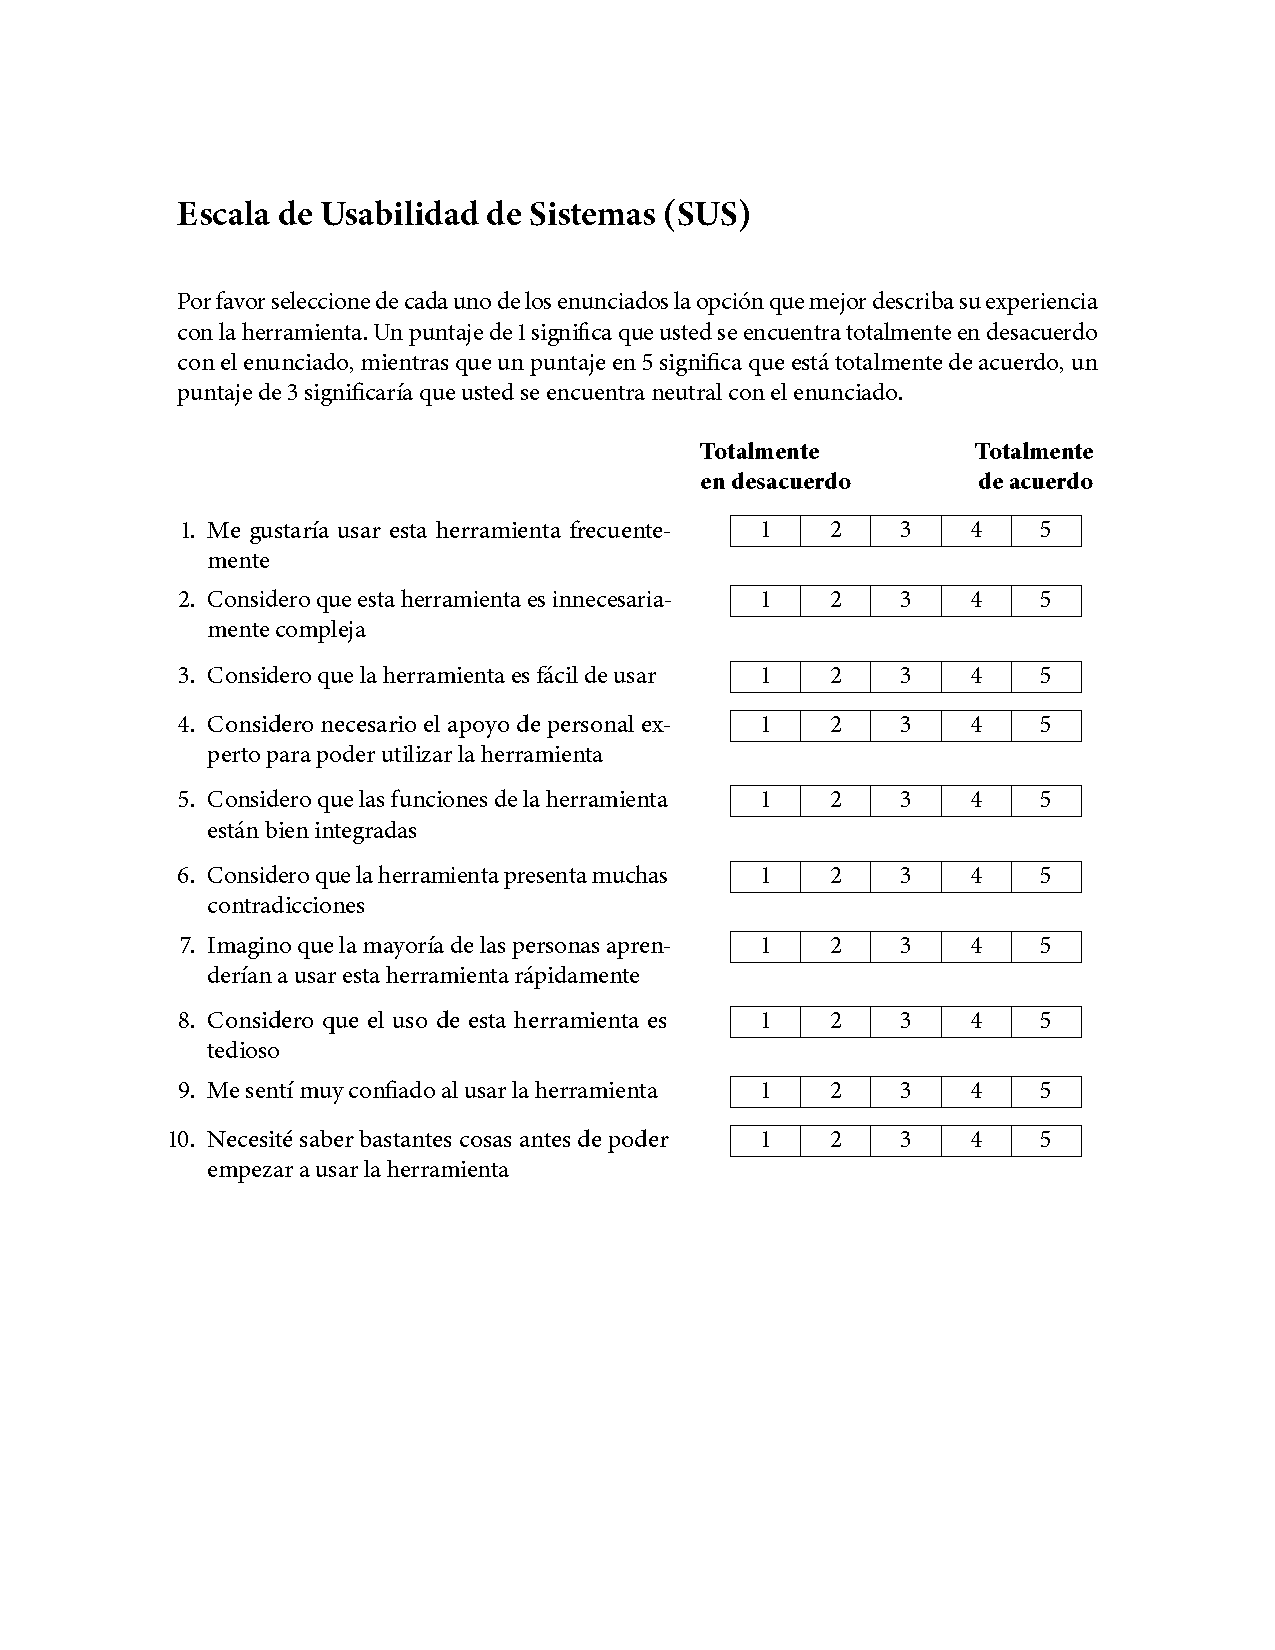
\includepdf[pages=1-3,pagecommand=\thispagestyle{plain}]{sus/sus.pdf}

\chapter{Certificación Comité de Ética y Bioseguridad}
\label{anexo:certificacion-comite-de-etica-y-bioseguridad}

\includepdf[pages=1-]{consentimiento/etica.pdf}

\chapter{Consentimiento informado}
\label{anexo:consentimiento}
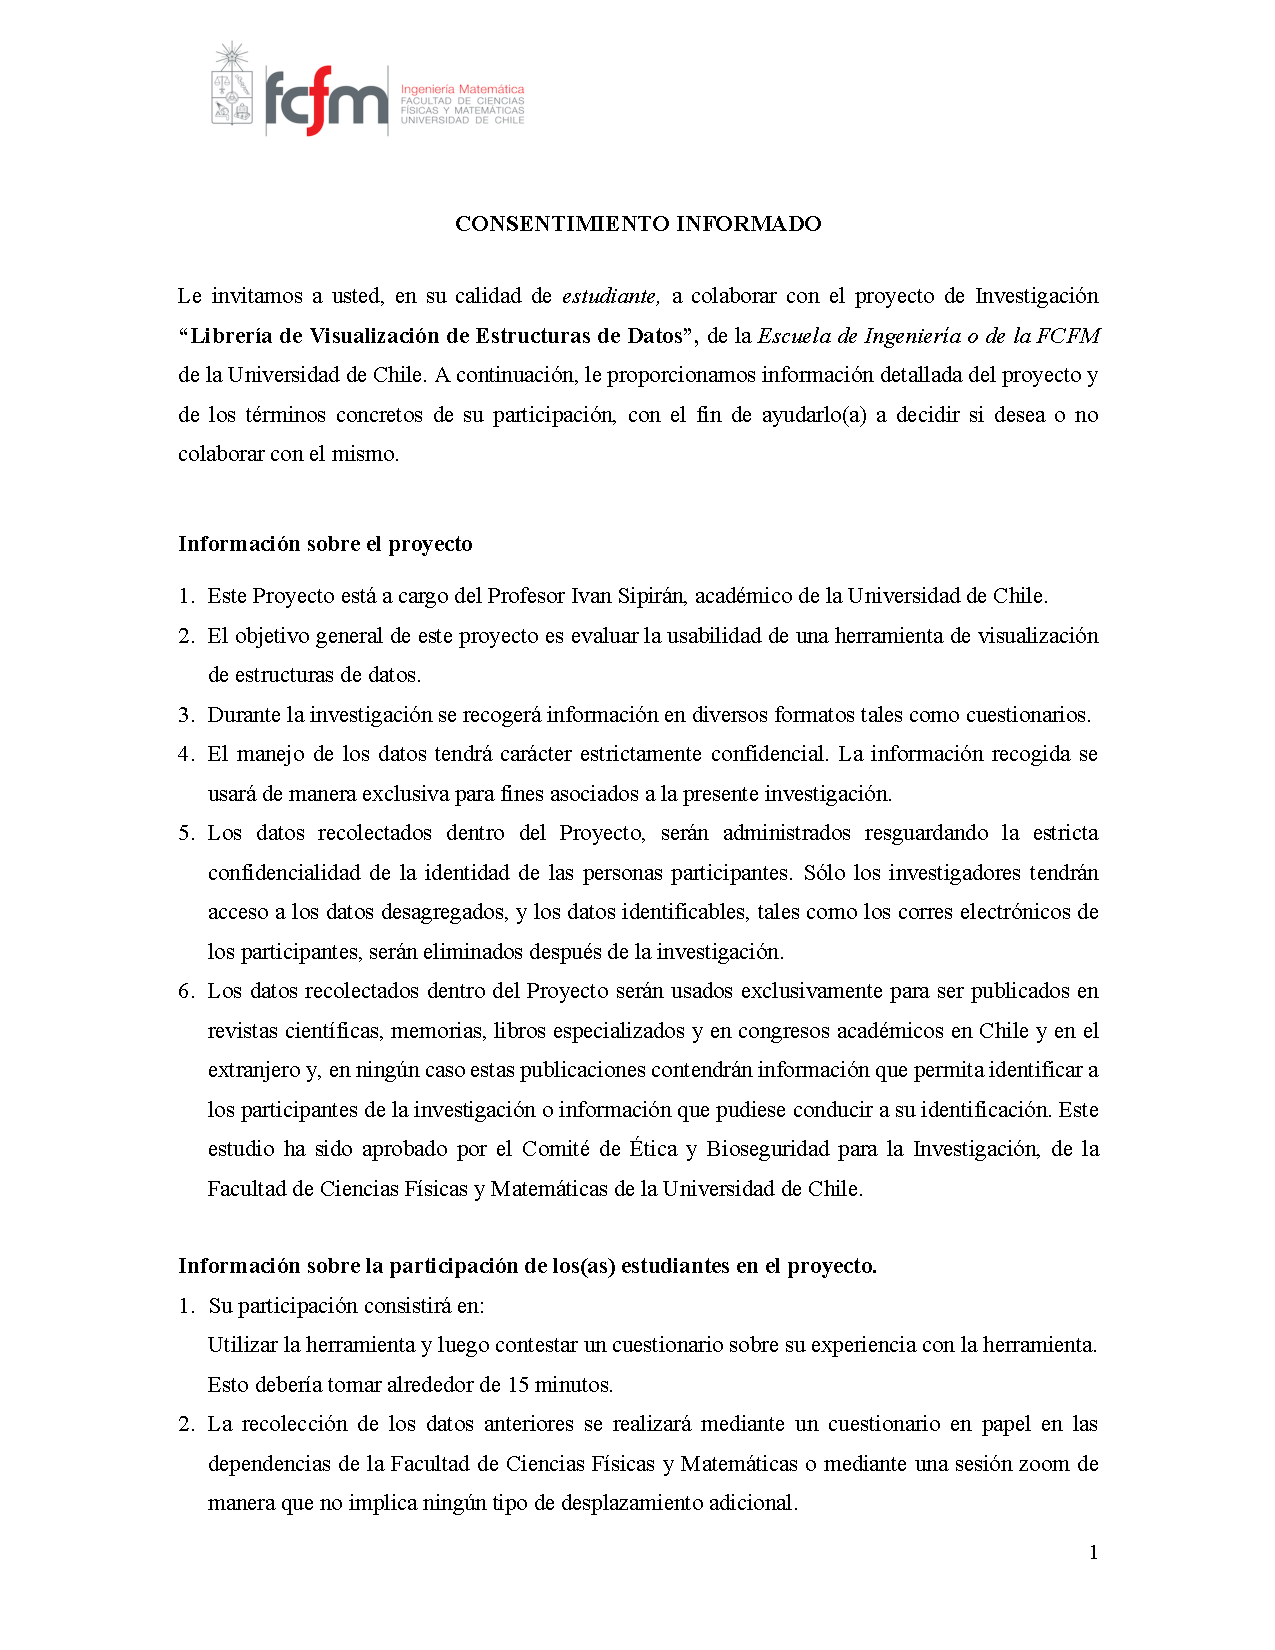
\includepdf[pages=1-3]{consentimiento/ConsentimientoinformadoSipiran.pdf}

\chapter{Respuestas}
\label{anexo:comentarios}

\section{¿Qué te gustó de la herramienta? ¿Por qué?}

\begin{enumerate}
    \item Si, fue entretenido ver como se movía cada parte de la lista y me permitió ver más fácilmente los errores
    \item Me gustó lo cómoda y fácil de usar la herramienta. No es necesario tanto conocimiento experto para usarla, y la visualización es muy intuitiva
    \item Los colores, son estéticamente agradables
    \item Que es bastante simple agregar a código que ya está escrito
    \item Logra mostrar claramente y paso a paso funciones que uno está creando. Esto ayuda enormemente a entender gráficamente lo que se está haciendo
    \item Pensando desde el punto de vista docente, me gustó porque me recordó la estructura de datos como la vi en cátedra por primera vez, las animaciones pueden ser aceledaras, lo cual me gustó. Además, el proceso que sigue la animación es bien claro y le hace completa justicia a la estructura de datos.
    \item Me gustó que fuera recorriendo el código y mostrando la visualización. Me gustó el tamaño y el color.
    \item Me gustó mucho que la visualización fuera mostrando la línea de código en la que estaba leyendo, pues ayuda enormemente a hallar errores en el código.
    \item Me gustó la idea de poder trabajar en tiempo real viendo como se construye la lista enlazada, más aún con la recursión que puede ser compleja de visualizar a primera.
    \item Me gustó que implementarlo requiera tan solo 2 líneas, es muy rápido.
    \item Ayuda a entender la construcción de una estructura paso a paso.
    \item Me gustó que fuera una visualización dinámica, es decir, muestra el proceso de los métodos llamados en la estructura de datos. Esto, porque me parece muy útil para entender lo que está sucediendo en la misma estructura.
\end{enumerate}

\section{¿Qué no te gustó de la herramienta? ¿Por qué?}

\begin{enumerate}
    \item Creo que para listas largas el tiempo en que va mostrando la lista se hace muy largo
    \item Nada, me gustó mucho
    \item No parece haber forma de quitar nodos
    \item Que no conocí de antemano las limitaciones, por lo tanto, algo que programé no servía (porque el nodo tenía dos "cabezas")
    \item No hay nada que realmente no me haya gustado. Lo único que podría mencionar es que la implementación de la herramienta se me hizo extraña, pero con la miniexplicación que se me presentó no tuve problema alguno.
    \item La visualización es buena, pero si le agrego algo de más de 6 elementos en la lista enlazada se pierde la visualización de algunas casillas. Por otro lado, si le paso listas un poco grandes como elemento a la lista, estas se representan algo más grandes que la casilla que le corresponde aunque esto último no es realmente una molestia, sino más bien una observación.
    \item No poder ajustar la velocidad y apariencia, o que no tuviera el formato del apunte.
    \item No le encontré ningún aspecto negativo
    \item 
    \item El uso de decoradores hace que sea un poco extraño para estudiantes del curso de algoritmos, pues no los he usado antes en este curso o en cursos anteriores.
    \item Es necesario que alguien explica que indica el puntero que va apuntando hacia abajo.
    \item No me gustó que al principio no entendí por qué quedaban más nodos de los que debe haber en la lista, al eliminar nodos.
\end{enumerate}

\section{¿Cómo podría ser mejor la herramienta?}

\begin{enumerate}
    \item Sería bueno añadir un parámetro de rapidez de visualización o algo de ese estilo
    \item Quizás no poner los paréntesis en el decorador "container" y que admita múltiples objetos en la visualización.
    \item Implementando la eliminación de nodos
    \item Listas muy largas no se muestran completas
    \item Si se logra expandir y que no solo funcione para listas enlazadas.
    \item Creo que solucionar de alguna manera la visualización para listas enlazadas para hasta 10 elementos sería bueno para la herramienta, pues pensando en la docencia al poder visualizar solo un par de datos es limitado.
    \item Personalización: Color, tamaño, velocidad, fuente, figura. En su defecto, predeterminado sea parecido al apunte.

          Muestras o ejemplos: visualizar por defecto dos o más posibilidades.

          Árboles: Suele ser la parte más difícil de entender, poder jugar con esto, serviría mucho más, pues las primeras listas se ven poco (poco relevante en comparación).

    \item Expandirse a más estructuras de datos o incluir etiquetas en la visualización
    \item Solamente aumentar sus usos, entendiendo que es la primera versión, le veo mucho potencial. Sentí que me faltó ver más usos, pero que fue para ver primeras impresiones.
    \item Que haya una opción para que no muestre todo el recorrido del código a la hora de agregar un elemento a la lista, que solo se agregue al final.
    \item Limitar que la figura se pueda salir del cuadro. Al tomarlo clickenado se puede sacar de lo visible de la pantalla.
    \item Cambiando el color de los nodos que ya no forman parte de la estructura principal, o sea, los que quedan libres. Por ejemplo, en el caso de ser eliminados de la lista.
\end{enumerate}

\end{appendices}
\end{document}
